%Vorlesung 17, 03.01.2011
\chapter{Lineare Programmierung}\label{chap:LP}
\section{Einführung in die Lineare Programmierung}
\begin{Bsp}
  \hspace{\parindent}Ein Molkereibetrieb hat zwei zentrale Sammelstellen. Eine erhält $15 m^3$, die andere $20 m^3$ Milch pro Tag. Des Weiteren hat der Betrieb drei Weiterverarbeitungsanlagen mit einer Kapazität von einmal $20 m^3$, einmal $15 m^3$ und einmal $10 m^3$ Milch pro Tag. Die Kosten für den Transport können wir Abbildung \vref{kap5Molkerei} entnehmen.
  
  \begin{figure}[htb]
    \centering
    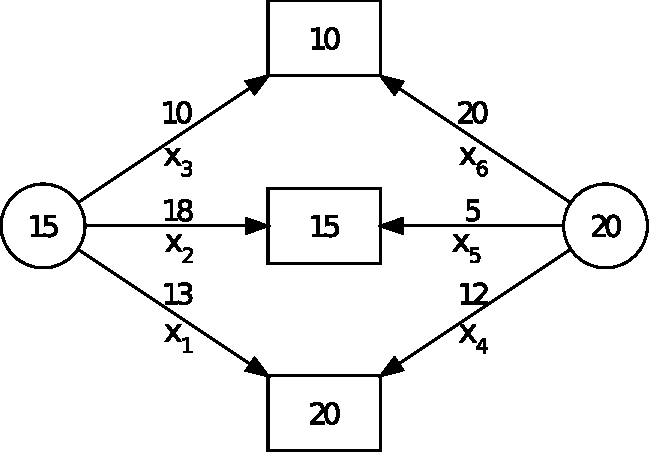
\includegraphics[scale=.66]{kap5Molkerei}
    \caption{Links und Rechts sehen wir die Sammelstellen, in der der Mitte die Weiterverarbeitungsanlagen der Molkerei. Die Kantengewichte entsprechen den Transportkosten in $Euro/m^3$.}
    \label{kap5Molkerei}
  \end{figure}

  Problem: minimiere die gesamten Transportkosten unter diesen Nebenbedingungen. Dazu formalisieren wir die Angaben aus Abbildung \vref{kap5Molkerei}, unsere Nebenbedingungen sind also:
  \begin{align*}
    x_1 + x_2 + x_3 &= 15 \\
    x_4 + x_5 + x_6 &= 20 \\
    x_1 + x_4 &\le 20 \\
    x_2 + x_5 &\le 15 \\
    x_3 + x_6 &\le 10
  \end{align*}
  Außerdem gelten Vorzeichenbedingungen, da wir einen Transport der Milch von einer Weiterverarbeitungsanlage zurück zu einer der Sammelstellen verhindern wollen. Es gilt also $x_1 \ge 0, \ldots, x_6 \ge 0$. Letztlich können wir die Zielfunktion aufstellen, die minimiert werden soll:
  \[ f(x_1, \ldots, x_6) = 13 x_1 + 18 x_2 +10 x_3 + 12 x_4 + 5 x_5 + 20 x_6 \]
\end{Bsp}

Betrachten wir \textit{Lineare Programmierung} (LP, \textit{linear programming}) oder auch \textit{Lineare Optimierung} (\textit{linear optimaziation}) allgemeiner. Man hat Variablen $x_1, \ldots, x_n$ und eine \textit{lineare Zielfunktion} (\textit{objective function}) $f : \mathbb{R}^n \to \mathbb{R}$ der Form $f(x_1, \ldots, x_n) : c_1 x_1 + \ldots + c_n x_n$.

Des Weiteren gibt es lineare \textit{Nebenbedingungen} (\textit{constraints}):
\[
  \begin{matrix}
    a_{1,1} x_1 &+& \ldots &+& a_{1,n} x_n &\le& b_1 \\
                & & \vdots\\
    a_{l,1} x_1 &+& \ldots &+& a_{l,n} x_n &\le& b_l\\
    a_{l+1,1} x_1 &+& \ldots &+& a_{l+1,n} x_n &\ge& b_{l+1}\\
                & & \vdots\\
    a_{r,1} x_1 &+& \ldots &+& a_{r,n} x_n &\ge& b_r\\
    a_{r+1,1} x_1 &+& \ldots &+& a_{r+1,n} x_n &=& b_{r+1}\\
                & & \vdots\\
    a_{k,1} x_1 &+& \ldots &+& a_{k,n} x_n &=& b_k\\
  \end{matrix}
\]
und Vorzeichenbedingungen (\textit{sign constraints)}: $x_1 \ge 0, \ldots x_s \ge 0, x_{s+1} \le 0, \ldots, x_t \le 0$.

Das zu lösende Problem ist nun, dass die Funktion $f(x_1, \ldots, x_n)$ unter Beachtung der Neben- und Vorzeichen"=Bedingungen zu minimieren oder zu maximieren ist.

Betrachten wir das Problem unseres Beispiels: als zusätzliche Bedingung bestimmen wir noch, dass die Milch in vollen Behältern von $1 m^3$ Fassungsvermögen transportiert werden muss, das heißt $f : \mathbb{Z}^n \to \mathbb{R}$. Probleme dieser Form nennt man \textit{Ganzzahlige Programmierung}. Für Lineare Optimierung gibt es Algorithmen, die in polynomieller Zeit arbeiten, ganzzahlige Optimierung ist NP-schwer.

Ein lineares Programm kann leicht auf eine \textit{kanonische Form} gebracht werden: minimiere $c_1 x_1 + \ldots + c_n x_n = c^T \cdot x$ unter den Nebenbedingungen
\[ \left.\begin{matrix} a_{1,1} x_1 &+ \ldots +& a_{1,n} x_n &\le b_1 \\ \vdots & \vdots & \vdots & \vdots \\ a_{k,1} x_1 &+ \ldots +& a_{k,n} x_n &\le b_k\end{matrix}\quad\right|\quad A \cdot x \le b \]
Dabei ist
\[ c = \begin{pmatrix}c_1 \\ \vdots \\ c_n\end{pmatrix} \text{, } x = \begin{pmatrix}x_1 \\ \vdots \\ x_n\end{pmatrix}  \text{, } b = \begin{pmatrix}b_1 \\ \vdots \\ b_k\end{pmatrix} \text{ und }  A = \begin{matrix}a_{1,1} &\ldots& a_{1,n} \\ \vdots & & \vdots \\ a_{k,1} &\ldots& a_{k,n}\end{matrix} \]
und $c^T$ natürlich der transponierte Vektor $c = \begin{pmatrix} c_1 & \ldots & c_n\end{pmatrix}$.

Zu beachten ist, dass alle Nebenbedingungen jetzt $\le$ enthalten und bei $A \cdot x \le b$ $\le$~komponentenweise zu verstehen ist. Hinzu kommen noch die Vorzeichenbedingungen $x_1 \ge 0, \ldots, x_n \ge 0$, "`$x \ge 0$"'.

Die \textit{Standardform} sieht wie folgt aus:
\begin{align*}
  min~c^T x &\quad \text{unter}\\
  A \cdot x = b \\
  x \ge 0
\end{align*}
wobei es für $x$ mehrere Lösungen gibt und die gesucht wird, die $c^T x$ minimiert.

\begin{Bew}[allgemeine Form $\to$ Standardform]
  \hspace{\parindent}Sollte das lineare Programm maximiert werden, ersetzen wir $max~c^T \cdot x$ durch $min~(-c)^T \cdot x$.
  Des Weiteren ersetzen wir alle Nebenbedingungen $a_{i,1} x_1 + \ldots + a_{i, n} x_n \le b_i$ durch $a_{i,1} x_1 + \ldots + a_{i,n} + s_i = b_i$, $s_i \ge 0$ beziehungsweise $a_{i,1} x_1 + \ldots + a_{i, n} x_n \ge b_i$ durch $a_{i,1} x_1 + \ldots + a_{i,n} + s_i = b_i$, $s_i \le 0$.
  $s_i$ ist dabei eine neue Variable, auch \textit{Schlupfvariable} (\textit{slack variable}) genannt.
  
  Alle Vorzeichenbedingungen werden zu $x_i \ge 0$ umgeformt. War zuvor die Vorzeichenbedingung $x_i \le 0$ angegeben, so wird $x_i$ überall durch $-x_i$ ersetzt. Gab es keine Vorzeichenbedingung für $x_i$, so ersetze überall $x_i$ durch $x_i^+ - x_i^-$, $x_i^+ \ge 0, x_i^- \ge 0$, wobei $x_i^+$ und $x_i^-$ neue Variablen sind.
\end{Bew}

\begin{Bsp}
  \begin{alignat*}{3}
    max~7x_1 + x_2 & &\quad\text{ unter N.B. }\\
    3 x_1 + 5 x_2 &\ge 0\\
    2 x_1 - x_2 &= 1 \\
    x_1 - 2 x_2 &\le 3 &\quad\text{ und V.B.}\\
    x_1 &\le 0
  \end{alignat*}
  Zunächst wird die Zielfunktion umgeformt zu $min~-7 x_1 - x_2$. Auch die Vorzeichenbedingung für $x_1$ müssen wir ändern, so dass die Zielfunktion zu $min~7 x_1 - x_2$ unter der Vorzeichenbedingung $x_1 \ge 0$ wird. Wir führen die Schlupfvariablen $s_1 \le 0$ und $s_2 \ge 0$ ein. Auch die Vorzeichenbedingung für $s_1$ formen wir zu $s_1 \ge 0$ um und ersetzen $s_1$ daher durch $-s_1$. Die Nebenbedingungen sehen nun wie folgt aus:
  \begin{align*}
    -3 x_1 + 5 x_2 - s_1 &= 0 \\
    -2 x_1 - x_2 &= 1 \\
    -x_1 - 2 x_2 + s_2 &= 3
  \end{align*}
  
  Die Standardform sieht abschließend wie folgt aus:
  \begin{alignat*}{3}
    min~7x_1 - x_2^+ + x_2^- & & \quad \text{ unter }\\
    -3x_1 + 5 x_2^+ - 5 x_2^- -s_1 &= 0 \\
    -2 x_1 - x_2^+ + x_2^- &= 1 \\
    -x_1 - 2x_2^+ + 2x_2^- + s_2 &= 3
    \end{alignat*}
    
  Als Matrix und Vektoren dargestellt sieht das wie folgt aus:
  \[ c = \begin{pmatrix}7 \\ -1 \\ 1 \\ 0 \\ 0\end{pmatrix} \text{, } x = \begin{pmatrix}x_1 \\ x_2^+ \\ x_2^- \\ s_1 \\ s_2 \end{pmatrix} \text{, } A = \begin{pmatrix} -3 & 5 & -5 & -1 & 0 \\ -2 & -1 & 1 & 0 & 0\\ -1 & -2 & 2 & 0 & 1\end{pmatrix} \text{ und }b = \begin{pmatrix} 0 \\ 1 \\ 3\end{pmatrix} \]
  \[ min~c^T \cdot x \text{ Nebenbedingung }A \cdot x = b \text{ Vorzeichenbedingung } x \ge 0\]
\end{Bsp}

\section{Geometrtie der Lineraren Programmierung}
Gegeben ist ein Lineares Programm. Der Bereich
\[ \{x = (x_1, \ldots, x_n) \mid x \text{ erfüllt Neben- und Vorzeichenbedingungen}\}\]
heißt \textit{zulässiger Bereich} (\textit{feasible region}). Ein Beispiel sehen wir in Abbildung \vref{kap5LPGeo1}.

\begin{figure}[htb]
  \centering
  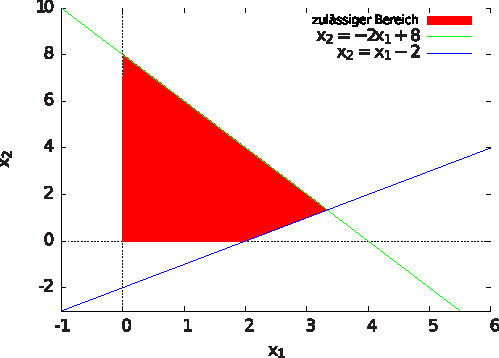
\includegraphics{kap5LPGeo1}
  \caption{Beispiel: Zulässige Bereich für die Nebenbedingungen $2x_1 + x_2 \le 8$, $x_1 - x_2 \ge 2$ und die Vorzeichenbedingungen $x_1, x_2 \ge 0$.}
  \label{kap5LPGeo1}
\end{figure}

\begin{Def}[konvexe Menge]
  \hspace{\parindent}Eine Menge $A$ heißt konvex genau dann, wenn $\forall x, y \in A, \lambda \in [0,1]$ gilt: $\lambda x + (1-\lambda) y \in A$. Das heißt mit $x, y \in A$ ist auch Strecke $\overline{xy} \subseteq A$.
\end{Def}

\begin{figure}[hbt]
  \centering
  \subfloat[\label{kap5konvexeBsp1}]{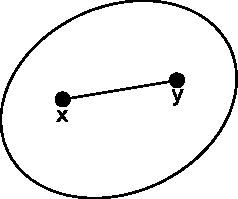
\includegraphics[scale=0.9]{kap5konvexeBsp1}}\hspace{2em}
  \subfloat[\label{kap5konvexeBsp2}]{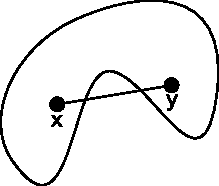
\includegraphics[scale=0.9]{kap5konvexeBsp2}}\hspace{2em}
  \subfloat[\label{kap5konvexeBsp3}]{
\includegraphics[scale=0.8]{kap5konvexeBsp3}}
  \caption{Drei Beispiele für Konvexe und nicht konvexe Figuren. Die Figur \subref{kap5konvexeBsp1} ist konvex, die beiden anderen sind es nicht.}
\end{figure}

\begin{Def}[Halbraum]
\hspace{\parindent}Eine Menge der Form: \[ \{ (x_1, \ldots, x_n) \mid a_1 x_1 + \ldots + a_n x_n \le b \} \quad a_1, \ldots a_n \in \mathbb{R}\] heißt Halbraum ("'Halbebene"' für $n=2$). Der zulässige Bereich eines linearen Programms ist ein Schnitt endlich vieler Halbräume, dass heißt er ist ein konvexes Polyeder (konvexes Polygon im Zweidimensionalen).
\end{Def}

\begin{figure}[htb]
  \centering
  \includegraphics[scale=.75]{kap5Wuerfel}
  \caption{Konvexes Polyeder in 3D mit den Nebenbedingungen $x_1 \ge 0$, $x_1 \le 1$, $x_2 \ge 0$, $x_2 \le 1$, $x_3\ge 0$ und $x_3 \le 1$: ein Würfel.}
  \label{kap5Wuerfel}
\end{figure}

%vorlesung 18
%vorlesung 18, 17.01.2010 (Fr)
Ein konvexes Polyeder kann entartet sein. Beispiele dafür sind Polyeder, die
\begin{itemize}
  \item leer sind, z.B. wenn sich die Gleichungen widersprechen
  \item aus einem einzelnen Punkt bestehen, wenn sich alle Halbebenen in nur einem Punkt schneiden
  \item Strecken sind
  \item Geraden sind, z.B. durch zwei gleiche Halbebenen mit unterschiedlichem Vorzeichen
  \item unbeschränkt sind
  \item \dots
\end{itemize}

\begin{Def}[Polytop]
  \hspace{\parindent}Ein beschränktes Polyeder nennt man auch \textit{Polytop}.
\end{Def}

\section{Wo nimmt eine lineare Zielfunktion ihr Minimum an?}
% Bemerkung: 45 minunten Erklärung. Daraus:
%
%Was bedeutet es einen Vektor zu transponieren (Skalarprodukt)?
%Zeichnung 18-1 und Beispiel aus vorhergehender Vorlesung mit verschiedenen Vektoren für c (Zeichnung 18-2) und antworten, was dann minimal ist. Die minimale Lösung hängt nicht von der Länge von c sonder nur von der Richtung von c ab.
%
%Ein beliebig dimensionaler Würfel hat die Nebenbedingungen $x_1 \ge 0$, $x_1 \le 1$, $\ldots$, $x_n \ge 0$, $x_n \le 1$. Er hat die Ecke $(1, 0, \ldots, 0)$. Allgemein hat er die Ecken $(\alpha_1, \ldots, \alpha_n)$ mit $\alpha_i \in \{0,1\}$. Das sind $2^n -  (2^\frac{1}{2})^N$ viele.
%
%Idee des Simplexalgorithmus.
% Es folgt die Formalisierung

\begin{Def}[Ecke (Extrempunkt) eines Polyeders]
  \hspace{\parindent}Ein Punkt $v$ eines konvexen Polyeders $P \subseteq \mathbb{R}^n$ heißt \textit{Ecke} (\textit{Extrempunkt}) genau dann, wenn er nicht auf einer Strecke $\overline{xy}$ liegt mit $x,y \in P$ und $x \neq v, y\neq v$.
\end{Def}

\begin{Lma}\label{kap5Lma1}
  \hspace{\parindent}Sei $P = \{x \in \mathbb{R}^n \mid A \cdot x \le b\}$ ein Polyeder, mit $A \in \mathbb{R}^{m \times n},~ b \in \mathbb{R}^m \text{ und } m \ge n$. Dann gilt: $v$ ist eine Ecke von $P$ genau dann, wenn es $n$ linear unabhängige Nebenbedingungen in $A x \le b$ gibt, für die in $v$ Gleichheit gilt.
\end{Lma}

\begin{Bew}[Lemma \ref{kap5Lma1}]
  \hspace{\parindent}\glq$\Rightarrow$\grq: Sei $v$ eine Ecke und $J \subset \{1, \ldots, m\}$ die Menge der linear unabhängigen Nebenbedingungen, bei denen für $v$ Gleichheit gilt: $J = \{j_1, \ldots, j_k\}$. Die zugehörigen Zeilenvektoren von $A$ sind $a_{j_1}, \ldots, a_{j_k}$. Angenommen $k < n$, dann existiert ein Vektor $t \in \mathbb{R}^n$ mit $a^T_{j_i} \cdot t = 0$ für $i=1, \ldots, k$. Das heißt $t$ ist orthogonal zu $a_{j_1}, \ldots, a_{j_k}$.
  \begin{figure}[htb]
    \centering
    \includegraphics[scale=0.5]{kap5BewLma1}
    \caption{$v$ liegt auf einer Strecke zwischen $v^+$ und $v^-$.}
    \label{kap5BewLma1}
  \end{figure}
  Definieren $v^+ = v + \gamma \cdot t$ und $v^- = v - \gamma \cdot t$. Dann ist $a^T_{j_i} \cdot v^{\pm} = a^T_{j_i} \cdot v \pm \gamma \cdot a^T_{j_i} t = a^T_{j_i} v = b_{j_i}$. Für ein $l \notin J$ mit $a_lv < b_l$ folgt dann $a_l v^+ < b_l,~ a_lv^- < b_l$ falls $\gamma > 0$ hinreichend klein. Also: $v^+, v^- \in P$. $v=\frac{1}{2}v^+ + \frac{1}{2} v^-$ liegt dann auf der Strecke zwischen $v^+$ und $v^-$, wie wir in Abbildung \vref{kap5BewLma1} sehen. $v$ kann nicht zeitgleich eine Ecke sein und auf einer Strecke zwischen zwei Punkten liegen, die zu $P$ gehören: Widerspruch.
  
  \glq$\Leftarrow$\grq: Sei $v$ keine Ecke von $P$. Daraus folgt $\exists v_1, v_2 \in P$ mit $v_1 \neq v_2$ und $v= \lambda v_1 + (1- \lambda) v_2$ und $0 < \lambda < 1$. Seien $a_{j_1} \ldots a_{j_n}$ Zeilenvektoren von $A$ bei denen bei $v$ Gleichheit gilt. Sei $B$ eine $n \times n$-Matrix, die $a_{j_1} \ldots a_{j_n}$ als Zeilenvektoren enthält. Da diese Vektoren linear unabhängig sind, ist $B$ regulär und somit invertierbar.
%  $B= \begin{pmatrix} a_{j_1} \\ \vdots \\ a_{j_n} \end{pmatrix}$ reguläre (daher invertierbare) $n \times n$-Matrix (weil alle Vektoren linear unabhängig sind?!).
  \[ \begin{pmatrix}b_{j_1} \\ \vdots \\ b_{j_n} \end{pmatrix} = b' = B v = \lambda (B v_1) + (1-\lambda)(B v_2) \]
  %  \[ \begin{pmatrix}b_{j_1} \\ \vdots \\ b_{j_n} \end{pmatrix} = b' = B v = \lambda \underbrace{(B v_1)}_{\le b' \text{ da } v_1 \in P} + (1-\lambda)\underbrace{(B v_2)}_{\le b'} \]
  
  Da $v_1 \in P$ wissen wir, dass $B v_1$ komponentenweise kleiner sein muss als $b'$. Das Gleiche gilt für $v_2$. Wäre eine der Komponenten echt kleiner, als $b'$, so wäre die Konvexkombination $B v = \lambda (B v_1) + (1-\lambda)(B v_2)$ in der entsprechenden Komponente echt kleiner als $b'$.  Damit ist $B v_1 = b'$ und $B v_2 = b'$. Daraus folgt $v_1 = B^{-1} b'$ und $v_2 = B^{-1} b'$, also $v_1 = v_2$. Dann muss jedoch $v$ eine Ecke sein, was jedoch im Widerspruch zu unserer ursprünglichen Annahme steht.
  %  Damit ist $B v_1 = b'$ und $B v_2 = b'$. Daraus folgt $v_1 = B^{-1} b'$ und $v_2 = B^{-1} b'$, also $v_1 = v_2$. Dann muss jedoch $v$ eine Ecke sein: Widerspruch.
\end{Bew}

\begin{Bem}
  \hspace{\parindent}Wenn $m < n$ ist, gibt es keine Ecken.
\end{Bem}

Falls (nur) $k$ der Ungleichungen die Form $a_1 v_1 + \ldots + a_n v_n = b$ haben und $n-k$ der Ungleichungen die Form $a_1 v_1 + \ldots + a_n v_n < b$, heißt die Menge der Punkte \textit{$(n-k)$"=dimensionale Facette} von $P$.

%Vorlesung 19, vom 10.01.10 (Mo)
Lösungen des linearen Programms finden wir also im zulässigen Bereich, das Minimum in Ecken (Extrempunkten) dieses Polyeders. Das lässt sich bei der Suche nach einer optimalen Lösung nutzen. 
Ohne Beschränkung der Allgemeinheit seien die Zeilenvektoren von $A$ linear unabhängig. Wenn die Zeilenvektoren von $A$ nicht linear unabhängig wären, gäbe es entweder Gleichungen die weggelassen werden könnten, oder sogar keine Lösung. Also ist $A$ vom Rang $m$. Daraus folgt: Es gibt $m$ linear unabhängige Spaltenvektoren. Diese bilden eine Basis des $m$-dimensionalen Bildraums. $J$ sei eine Menge von Spaltenvektoren aus $A$: $J = j_1 < \ldots < j_m$ und B eine $m \times m$-Matrix, die aus diesen Spalten besteht. Falls die Spaltenvektoren eine Basis bilden, sei
\[ a = B^{-1} \cdot b \quad \in \mathbb{R}^m \]
Daraus folgt $B \cdot a = b$. Dann definiere $x \in \mathbb{R}^n$ durch $x_{j_i} = a_i$ mit $ i=1, \ldots, m$ und $x_l = 0$ für $l \notin J$.
\[ x = \begin{pmatrix}0 \\ \vdots \\ 0 \\ a_{j_1} \\ 0 \\ \vdots \\ 0 \\ a_{j_2} \\ \vdots \end{pmatrix} \]
$x$ erfüllt die Nebenbedingungen des linearen Programms, denn
\[ A \cdot x = A \cdot \begin{pmatrix} 0 \\ \vdots \\ 0 \\ a_{j_1} \\ 0 \\ \vdots \\ 0 \\ a_{j_2} \\ \vdots \end{pmatrix} = B \cdot a = b\]
$x$ heißt \textit{Basislösung} des linearen Programms.
Falls $x$ auch die Vorzeichenbedingungen des linearen Programms erfüllt, heißt es \textit{zulässige Basislösung} (bfs, \textit{basic feasible solution}.

Fassen wir einmal zusammen: Zum lineare Programm $ A \cdot x = b$, $x \ge 0$ mit der $m \times n$-Matrix $A$ ist die zulässige Basislösung (bfs) ein Vektor. Dazu wählen wir aus $A$ $m$ linear unabhängige Spaltenvektoren aus und bilden mit diesen eine invertierbare $m \times m$-Matrix. Diese Matrix ergibt zusammen mit unserem Vektor $b$ ein Gleichungssystem, das wir lösen (da $B$ invertierbar ist, ist das einfach). Die Komponenten des als Lösung gefunden Vektors können wir einzelnen Spalten von $A$ zuordnen. Wir konstruieren nun einen $n$"=dimensionalen Vektor, der für jede Spalte von $A$ eine Komponente unseres Lösungsvektors enthält oder $0$ ist, wenn die entsprechende Spalte keiner Komponente der Lösung des Gleichungssystem zugeordnet ist. Dieser $n$"=dimensionale Vektor stellt eine Basislösung dar. Entspricht dieser Vektor auch den Vorzeichenbedingungen, so handelt es sich um eine zulässige Basislösung.

In einer so konstruierten Basislösung sind $m$ Nebenbedingungen und $n-m$ Vorzeichenbedingungen durch Gleichheit erfüllt.

\begin{Satz}
  \hspace{\parindent}Im Linearen Programm $min~c^Tx$, $Ax = b$, $x \ge 0$ ist $w \in \mathbb{R}^n$ eine bfs genau dann, wenn $w$ eine Ecke des Polyeders der zulässigen Lösungen $F$ ist.
\end{Satz}

Auf Grund der Komplexität des Beweises sei hier nur die Beweisidee kurz skizziert: $w$ ist bfs $\Leftrightarrow$ $w$ erfüllt $m$ Nebenbedingungen mit Gleichheit und $n-m$ Vorzeichenbedingungen mit Gleichheit. $m + n - m = n$ $\Leftrightarrow$ $w$ ist Ecke, ähnlich wie der Beweis von Lemma \ref{kap5Lma1}.

\begin{Koro}
\hspace{\parindent}Es gibt höchstens $\binom{n}{m}$ Ecken des zulässigen Bereichs. Also gibt es höchstens $\binom{n}{m}$-mal eine Auswahl von $j_1 \ldots j_m \in \{ 1, \ldots, n \}$. Daher gibt es höchstens $\binom{n}{m}$ viele bfs.
\end{Koro}

\begin{Satz}
  \hspace{\parindent}Das Lineare Programm $min~c^Tx$, $Ax = b$, $x \ge 0$ habe den zulässigen Bereich $F$, $p\in F$. Dann ist entweder $c^Tx$ auf $F$ nach unten unbeschränkt, oder es existiert eine Ecke $v$ von $F$ mit $c^Tv \le c^T p$.
\end{Satz}

Das heißt falls $c^T x$ sein Minimum auf $F$ annimmt, wird es bei einer Ecke von $F$ angenommen. Es ist möglich, dass eine Facette von $F$ oder sogar $F$ komplett das Minimum von $c^T x$ annimmt. In jedem dieser Fälle ist aber eine Ecke enthalten.

Auch hier geben wir nur die Beweisidee an: Wir wählen zunächst einen Punkt $p \in F$. Ein Beispiel sehen wir in Abbildung \vref{kap5PAusF}.

\begin{figure}[hbt]
  \centering
  \includegraphics[scale=.66]{kap5PAusF}
  \caption{Ein Punkt $p$ aus einem zulässigen Bereich $F$ eines linearen Programms.}
  \label{kap5PAusF}
\end{figure}

Falls $p$ keine Ecke ist, muss es zwei Punkte $u$ und $v$ geben, mit $u,v \in F$, so dass $p$ auf einer Geraden $g$ liegt, die auch durch die Punkte $u$ und $v$ geht. Abbildung \vref{kap5GeradeUPV} veranschaulicht das.

Auf der Geraden $g$ in Richtung $\overrightarrow{uv}$ ist $c^Tx$ strikt monoton fallend oder strikt monoton wachsend, da $c^Tx$ eine lineare Funktion ist. Solche $u, v$ existieren, es sei denn $c^T x$ ist überall konstant, dann wäre sie aber auch überall minimal. Ohne Beschränkung der Allgemeinheit gehen wir davon aus, dass $g$ in Richtung  $\overrightarrow{uv}$ monoton fallend ist (andernfalls vertauscht man $u$ und $v$). Angenommen wir verfolgen $g$, treffen jedoch nicht auf den Rand von $F$. Dann ist $F$ unbeschränkt, dann ist auch $c^T x$ in diese Richtung unbeschränkt. Andernfalls treffen wir auf den Rand von $F$ in $p'$ und $c^T p' \le c^Tp$. $p'$ liegt dann auf einer niedrigerdimensionalen Facette von $F$, siehe auch Abbildung \vref{kap5GeradeUPV}. Diese Verfahren wiederholen wir rekursiv, bis wir eine Facette der Dimension $0$ finden. Facetten der Dimension $0$ sind Ecken.

\begin{figure}[htb]
  \centering
  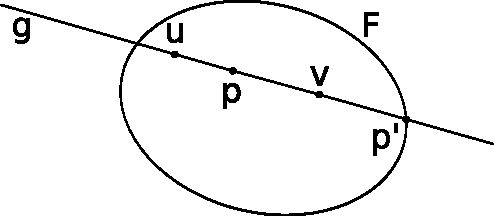
\includegraphics[scale=.66]{kap5GeradeUPV}
  \caption{Wenn $p$ keine Ecke von $F$ ist, muss es zwei Punkte $u, v \in F$ geben, durch die eine Gerde $g$ führt, auf der auch $p$ liegt.}
  \label{kap5GeradeUPV}
\end{figure}

Das Vorgehen, das in der Beweisidee skizziert wurde, werden wir uns später genauer ansehen. Es ist das \textit{Simplex"=Verfahren}.

%Solche $u,v$ gibt es, es sei denn $c^Tx$ ist überall konstant, also $\equiv 0$ daraus folgt: Satz gilt sowieso. (Falls es konstant bleibt, bleibt es immer konstant. Wir haben es mit einer linearen Funktion zu tun. Das heißt wenn sie in alle Richtungen konstant ist, ist sie insgesamt konstant und $c^T \cdot v$ ist überall minimal. Sonst findet man immer eine Richtung, in die sie fällt oder steigt.) Das heißt auf der Geraden durch $u,v$
%  \begin{enumerate}\renewcommand{\theenumi}{\alph{enumi}}
%    \item wir treffen den Rand von $F$ in $p_1$ und $c^T p_< \le c^Tp$. $p_1$ liegt dann auf einer niedrigerdimensionalen Facette von $F$ und wir wenden das Verfahren rekursiv darauf an, bis wir eine Facette der Dimension 0 haben: eine Ecke.
%    \item wir treffen den Rand nicht, $F$ ist unbeschränkt. Falls $c^T x$ kleiner wird, wir es immer kleiner und ist nach unten unbeschränkt.
%  \end{enumerate}

\section{Geometrische Erklärung}
Ein lineares Programm, dass eine zulässige Lösung hat, hat einen zulässigen Bereich $F$, der sich aus den Neben- und Vorzeichenbedingungen ergibt. Die Zielfunktion lässt sich als Vektor $c$ darstellen. Stellen wir uns vor, dass durch $c$ eine Gerade $g$ führt. Nun kann man $F$ auf diese Gerade projizieren, und den Punkt $c^Tx^*$ bestimmen, an dem $c^Tx$ innerhalb des zulässigen Bereichs $F$ minimiert wird. Abbildung \vref{kap5GeometrischeErkl} veranschaulicht die geometrische Erklärung der linearen Programmierung.

\begin{figure}[htb]
  \centering
  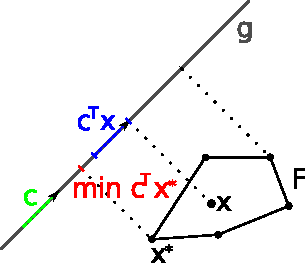
\includegraphics[scale=1.25]{kap5GeometrischeErkl}
  \caption{Zur geometrischen Erklärung von linearer Programmierung betrachten wir uns $F$, $c$, eine Gerade $g$ durch $c$ und eine Projektion von $F$ auf $g$.}
  \label{kap5GeometrischeErkl}
\end{figure}

Davon ausgehend würde ein "`einfacher"' Algorithmus wie folgt vorgehen, um ein lineares Programm zu lösen:
\begin{itemize}
  \item stelle fest, ob $c^Tx$ auf $F$ beschränkt.
  \item falls ja, inspiziere alle Ecken von $F$, nehmen die, wo $c^Tx$ minimal.
\end{itemize}

Dieser Algorithmus hat leider exponentielle Laufzeit: es gibt $\binom{n}{m}$ Ecken, wobei $n$ die Dimension und $m$ die Anzahl der Nebenbedingungen ist. Die Laufzeit wird maximal, wenn $m = \frac{n}{2}$:
\[\binom{n}{\frac{n}{2}} = \frac{n \cdot (n-1) \cdot \ldots \cdot (\frac{n}{2} +1)}{\frac{n}{2} \cdot (\frac{n}{2} -1) \cdot \ldots \cdot 2 \cdot 1} \ge 2^{\frac{n}{2}} = \sqrt{2}^n = 1,41\ldots^n \]
Das ist exponentiell.

Der Simplex"=Algorithmus ist schneller, jedoch im schlechtesten Fall immer noch exponentiell. In der Praxis spielt das selten eine Rolle, da der schlechteste Fall hier nur selten auftritt. Anfang der achtziger Jahre wurde gezeigt, dass sich lineare Programmierung sogar echt in polynomieller Zeit lösen lässt. Wir wolle uns im Folgenden den Simplex"=Algorithmus näher anschauen, mit einem konkreten Beispieldurchlauf beginnend.

\section{Der Simplex"=Algorithmus}
\subsection{Beispieldurchlauf des Simplex"=Algorithmus}
\begin{Bsp}
  \begin{align*}
    \text{maximiere } & 5x_1 + 4x_2 + 3x_3 \\ 
    \text{Nebenbedingungen } & 2x_1 + 3x_2 + x_3 \le 5\\
    & 4x_1 + x_2 + 2x_3 \le 11\\
    & 3x_1 + 4x_2 + 2x_3 \le 8\\
    \text{Vorzeichenbedingungen } & x\ge 0
  \end{align*}
  
  Standardform durch Schlupfvariablen $x_4, x_5, x_6$:
  \[ min~c^Tx \quad Ax = b \quad x \ge 0 \]
  \[ b=\begin{pmatrix} 5 \\ 11 \\ 8 \end{pmatrix} \quad x=\begin{pmatrix} x_1 \\ \vdots \\ x_6 \end{pmatrix} \quad A=\begin{pmatrix} 2 & 3 & 1 & 1 & 0 & 0 \\ 4 & 1 & 2 & 0 & 1 & 0 \\ 3 & 4 & 2& 0 & 0 & 1 \end{pmatrix} \quad c=\begin{pmatrix} -5 \\ -4 \\ -3 \\ 0 \\ 0 \\ 0 \end{pmatrix}\]
  
  Wir formen das um, so dass wir folgendes erhalten:
  \begin{align*}
    x_4 &= \hphantom{1}5 -2x_1 -3x_2 -\hphantom{2}x_3\\
    x_5 &= 11 -4x_1 -\hphantom{3}x_2 -2x_3 \\
    x_6 &= \hphantom{1}8 -3x_1 -4 x_2 -2 x_3 \\
    z &= \hphantom{11} -5x_1 -4x_2 - 2x_3
  \end{align*}
  
  Diese Form der Darstellung von Variablen (hier $x_4$, $x_5$, $x_6$ und $z$) durch andere Variable nennt man auch \textit{Dictionary}. $z$ ist hier bereits in eine Form gebracht, bei der es zu minimieren ist. Genau genommen werden die Basisvariablen und die Zielfunktion dabei durch Nichtbasisvariablen dargestellt.
  
  Wir versuchen eine erste zulässige Basislösung zu finden: $x_1 = x_2 = x_3 = 0$. Daraus folgt $x_4 =5$, $x_5 = 11$ und $x_6 = 8$. Wir haben Glück, diese Basislösung entspricht auch den Vorzeichenbedingungen. Daher
  \[ \text{bfs} = \begin{pmatrix} 0 \\ 0 \\ 0 \\ 5 \\ 11 \\ 8 \end{pmatrix} \]
  
  %vorlesung 20 vom 14.01.2011 (Fr)
  Die bfs besteht aus den Spalten $4$, $5$ und $6$.
  \[ A= \begin{pmatrix} 2 & 3 & 1 & 1 & 0 &0 \\ 4 & 1 & 2 & 0 & 1 & 0 \\ 3 & 4 & 2 & 0 & 0 & 1\end{pmatrix} \]
  In der ersten Zeile der Matrix wurde die Schlupfvariable $x_4$ addiert, in der zweiten Zeile $x_5$ und in der dritten Zeile $x_6$. Die letzten drei Spalten sind die Spalten, die wir zur Lösung ausgewählt haben, auf Grund ihrer einfachen Form. Der Wert der Zielfunktion ist $z=0$.
  
  Dies kann verbessert werden durch Vergrößerung von $x_1$ um ein minimales $\Theta$. $x_2, x_3$ bleiben dabei $0$. Wir setzen $x_1$ also auf einen Wert $\Theta$ und erhöhen ihn soweit, dass die Vorzeichenbedingungen nicht verletzt werden. $\Theta$ lässt sich wie folgt berechnen:
\[
  \left.
    \begin{matrix}
        x_4 = 5 - 2\Theta &&\Theta \le \frac{5}{2}\\
        x_5 = 11 - 4 \Theta &\quad \ge 0 \quad& \Theta \le \frac{11}{4}\\
        x_6 = 8-3 \Theta && \Theta \le \frac{8}{3}
      \end{matrix}
    \right\}
    \Theta = \frac{5}{2} \text{ funktioniert}
  \]
  Alle drei Bedingungen sind und"=verknüpft, müssen also alle erfüllt sein. Daher wählen wir das Minimum aus und setzten $\Theta = \frac{5}{2}$.

  Daraus folgt eine neue bfs, wobei $x_1 = \Theta$ wird und $x_4 = 0$. Die neue bfs beinhaltet die Spalten $1, 5, 6$. Die neue bfs sieht wie folgt aus:
  \[ \text{bfs} = \begin{pmatrix} \frac{5}{2} \\ 0 \\ 0 \\ 0 \\ 1 \\ \frac{1}{2} \end{pmatrix} \quad z = - \frac{25}{2}\]
  
  Man kann nun ein neues Dictionary aufstellen. Dazu stellen wir die Gleichung von $x_4$ nach $x_1$ um. In die Gleichungen für $x_5$, $x_6$ und $z$ setzen wir jetzt diese Gleichung für $x_1$ ein, also zum Beispiel $x_5 = 11 - 4 (\frac{5}{2} - \frac{3}{2} x_2 - \frac{1}{2} x_3 - \frac{1}{2} x_4) - x_2 -2 x_3$. Das neue Dictionary sieht dann wie folgt aus:
  \begin{align*}
    x_1 &= \frac{5}{2} - \frac{3}{2} x_2 - \frac{1}{2} x_3 - \frac{1}{2} x_4 \\
    x_5 &= 1 + 5 x_2 + 2x_4\\
    x_6 &= \frac{1}{2} + \frac{1}{2} x_2 - \frac{1}{2} x_3 + \frac{3}{2} x_4 \\
    z &= - \frac{25}{2} + \frac{7}{2} x_2 - \frac{1}{2}  x_3 + \frac{5}{2} x_4
  \end{align*}

  Jetzt erhöhen wir $x_3$ um $\Theta$:
  \[ \left. \begin{matrix} x_1 = & \frac{5}{2} & - & \frac{1}{2} \Theta\\ x_5 = & 1 \\ x_6 = & \frac{1}{2} & - & \frac{1}{2} \Theta\end{matrix}\quad \right\} \ge 0 \qquad \begin{matrix}\Theta \le 5 \\\strut\\ \Theta \le 1 \end{matrix}\]
  Daraus folgt $x_3 : = 1$ und wieder eine neue bfs:
  \[ \text{bfs} = \begin{pmatrix}2 \\ 0 \\ 1 \\ 0 \\ 1 \\ 0\end{pmatrix} \]
  Aus einer neuen bfs folgt ein neues Dictionary, wir stellen die Gleichung für $x_6$ nach $x_3$ um:
  \begin{align*}
    x_1 &= \\
    x_3 &= 1 + x_2 + 3 x_4 - 2 x_6 \\
    x_5 &= \\
    z &= -\frac{25}{2} + \frac{7}{2} x_2 - \frac{1}{2} (1 + x_2 + 3 x_4 - 2x_6) + \frac{5}{2} x_4\\
      &= -13 + 3 x_2 + x_4 + x_6
  \end{align*}

  Die Zielfunktion $z = -13 + 3 x_2 + x_4 + x_6$ ist minimal genau dann, wenn $x_2 = x_4 = x_6 = 0$ gesetzt wird. Wir haben das Optimum gefunden. Die zugehörige bfs ist
  \[ \text{bfs} = \begin{pmatrix} 2 \\ 0 \\ 1 \\ 0 \\ 1 \\ 0 \end{pmatrix} \]
  Lassen wir die Schlupfvariablen weg, so erhalten wir die Lösung des ursprünglichen Linearen Programms. Die Lösung des ursprünglichen Linearen Programms ist also
  \[ \begin{pmatrix} x_1 \\ x_2 \\ x_3 \end{pmatrix} = \begin{pmatrix} 2 \\ 0 \\ 1 \end{pmatrix} \]
\end{Bsp}

\subsection{Tableau-Darstellung}
Das Simplex"=Verfahren lässt sich besser veranschaulichen, wenn man ein Tableau benutzt. Dazu schreibt man die Matrix $A$ neben den Vektor $b$ und darunter die Zielfunktion $z$:
\begin{center}
\begin{tabular}{ccccc|l}
%  $x_1$ & $x_2$ & $x_3$ & $x_4$ & $\ldots$ & \\\hline
  & & & & & \multirow{5}{*}{\rotatebox{90}{Vektor $b$}}\\
  & & & & &\\
   & \multicolumn{3}{c}{Marix $A$} & \\
  & & & & &\\
  & & & & &\\\hline
  & \multicolumn{3}{c}{Zielfunktion $z$} & & Wert von $z$
\end{tabular}
\end{center}

Bringen wir also unser Beispiel in diese Form:
\begin{center}
\begin{tabular}{>{$}r<{$}>{$}r<{$}>{$}r<{$}>{$}r<{$}>{$}r<{$}>{$}r<{$}|>{$}r<{$}}
  2 & 3 & 1 & 1 & 0 &0 & 5 \\
  4 & 1 & 2 & 0 & 1 & 0 & 11\\
  3 & 4 & 2 & 0 & 0 & 1 & 8\\\hline
  5 & 4 & 3 & 0 & 0 & 0 &0
\end{tabular}
\end{center}
Die Spalten entsprechen dabei natürlich $x_1$ bis $x_6$ gefolgt vom Vektor $b$.

Als \textit{Pivot"=Schritt} bezeichnen wir den Schritt von einer bfs zur nächsten. Ein Pivot"=Schritt wird wie folgt durchgeführt, wobei wir diesen Prozess rekursiv wiederholen:
\begin{enumerate}
  \item finde das Maximum der untersten Zeile. Die Spalte mit dem Maximum nennen wir \textit{Pivot"=Spalte}. Falls das Maximum kleiner oder gleich $0$ sein sollte, sind wir fertig und haben eine optimale Lösung gefunden, andernfalls:
  \item Für jede Zeile deren Eintrag $r$ in der Pivot"=Spalte positiv ist betrachten wir Eintrag $s$ in der rechtesten Spalte. Wir bestimmen die Zeile mit dem Kleinstem $\frac{s}{r}$, als \textit{Pivot"=Zeile}.
  \item Als \textit{Pivot"=Zahl} bezeichnen wir den Eintrag in der Pivot"=Spalte und Pivot"=Zeile. Jeder Eintrag der Pivot"=Zeile wird nun durch die Pivot"=Zahl dividiert.
  \item Von den übrigen Zeilen subtrahieren wir ein geeignetes Vielfaches der "`umgeformten"' Pivot"=Zeile (wie beim Gaußschen Eliminationsverfahren), so dass deren Einträge in der Pivot"=Spalte $0$ werden.
\end{enumerate}

Bei einem Pivot"=Schritt wird also die Lösung des Linearen Programms verbessert, in dem eine der Nichtbasisvariablen erhöht wird. Dadurch fällt eine Basisvariable raus und die erhöhte Nichtbasisvariable wird dafür Teil der neuen Basis und somit Teil der bfs. 

Im ersten Schritt haben wir also Spalte $x_1$ markiert, im zweiten Schritt die erste Zeile. Die Pivot"=Zahl steht also in der ersten Spalte und ersten Zeile. Wir teilen die erste Zeile spaltenweise (komponentenweise) durch $2$ und subtrahieren diese neue Zeile viermal von der zweiten und dreimal von der dritten Zeile. Wer erhalten nun folgendes Tableau:
\begin{center}
\begin{tabular}{>{$}r<{$}>{$}r<{$}>{$}r<{$}>{$}r<{$}>{$}r<{$}>{$}r<{$}|>{$}r<{$}}
  1 & \nicefrac{3}{2} & \nicefrac{1}{2} & \nicefrac{1}{2} & 0 &0 & \nicefrac{5}{2} \\
  0 & -5 & 0 & -2 & 1 & 0 & 1\\
  0 & -\nicefrac{1}{2} & \nicefrac{1}{2} & -\nicefrac{3}{2} & 0 & 1 & \nicefrac{1}{2}\\\hline
  0 & -\nicefrac{7}{2} & \nicefrac{1}{2} & -\nicefrac{5}{2} & 0 & 0 & -\nicefrac{25}{2}
\end{tabular}
\end{center}
Das Maximum der letzten Zeile ist $\frac{1}{2} > 0$. Unsere neue Pivot"=Spalte ist also die dritte Spalte. Neue Pivot"=Zeile ist also die dritte Zeile. Das nächste Tableau sieht also wie folgt aus:
\begin{center}
\begin{tabular}{>{$}r<{$}>{$}r<{$}>{$}r<{$}>{$}r<{$}>{$}r<{$}>{$}r<{$}|>{$}r<{$}}
  1 & 2 & 0 & 2 & 0 & -1 & 2 \\
  0 & -5 & 0 & -2 & 1 & 0 & 1 \\
  0 & -1 & 1 & -3 & 0 & 2 & 1 \\\hline
  0 & -3 & 0 & -1 & 0 & -1 & - 13
\end{tabular}
\end{center}
In der letzten Zeile gibt es kein Maximum, dass größer oder gleich null ist. Wir haben also eine optimale Lösung gefunden. Wir können die Lösung direkt aus dem Tableau ablesen (anhand der Spalten"=Einheitsvektoren):
\[ \text{bfs } = \begin{pmatrix} 2 \\ 0 \\ 1 \\ 0 \\ 1 \\ 0 \end{pmatrix} \]

\subsection{Einzelprobleme des Simplex"=Algorithmus}
Wir wollen noch Einzelprobleme des Simplex"=Verfahrens betrachten:
\begin{enumerate}
  \item Initialisierung: Wie findet man eine geeignete erste bfs und dem entsprechend das Start"=Dictionary?
  \item Iteration: Findet man immer eine geeignete \textit{Eintrittsvariable} zum Erhöhen und eine \textit{Austrittsvariable}, die stattdessen herausfällt?
  \item Terminierung: Könnte die Methode in eine unendliche Schleife geraten?
\end{enumerate}

\subsubsection{Initialisierung}
Wir wählten im Beispiel
\[ x_{n+i} = b_i - \sum_{j=1}^{n} a_{i,j} x_j \qquad i= 1, \ldots, m \]
als Dictionary. Das heißt wir hatten $(x_1, \ldots, x_n, b_1, \ldots, b_m) = (0, \ldots, 0, b_1, \ldots, b_m)$ als Anfangslösung. Das ist allerdings nur zulässig, falls $b_i \ge 0$ für $i = 1, \ldots, m$. Das ist im Allgemeinen aber nicht der Fall.

%Andernfalls können wir dieses Problem wie folgt beheben:
%Angenommen das lineare Programm liegt in kanonischer Form $\text{min }c^Tx \quad A x \le b \quad x \ge 0$ vor. Wir suchen ein Hilfsproblem mit einer zusätzlichen Variable $x_0$ und minimieren $x_0$, wobei das Hilfsproblem die Nebenbedingungen
%\[ \sum_{j=1}^{n} a_{i,j} x_{j} - x_0 \ge b_i \]
%und die Vorzeichenbedingungen $x_0, x_1, \ldots \ge 0$ hat. Dann sind die folgenden drei Aussagen äquivalent:
%\begin{itemize}
%  \item Das ursprüngliche Problem hat überhaupt eine zulässige Lösung
%  \item Das Hilfsproblem hat eine zulässige Lösung mit $x_0 = 0$
%  \item Das Hilfsproblem hat den optimalen Wert $0$.
%\end{itemize}

% Vorlesung 21 vom 17.01.2011 (Mo)
%Simplex"=Algorithmus geht aus von eine Lösung und verbessert diese, so lange es geht. Hangelt sich dabei von Ecke zu Ecke.
%
%Dictionary: Basisvariablen als Linearkombination der anderen Variablen. Zielfunktion auch.
%Pivotschritt: Verbessern der Lösung, durch erhöhen einer der Basisvariablen. Dadurch fällt eine Basisvariable raus, dadurch, dass Ihr Wert null wird, die Basisvariable tritt dann in die Lösung ein.
%Matrix $A = m \times n$. Basisvariablen: Spaltenvektoren, die Basis bilden, das linear unabhängig. Schlupfvariablen bilden am Anfang immer eine Basislösung, aber nicht immer eine zulässige Basislösung.
%
%Probleme:
%\begin{enumerate}
%  \item Start-BFS finden: Initialisierung
%  \item Iteration: finde geeignete Austritts und Eintrittsvariablen
%  \item Terminierung: endet die Simplex"=Methode immer oder kann sie in eine unendliche Schleife laufen?
%\end{enumerate}
%
%Initialisierung:
%im Beispiel kein Problem, weil $b_j \ge 0 \quad j=1, \ldots, m$ im Allgemeinen ist das aber nicht der Fall.

Das Problem lässt sich jedoch leicht lösen. Wir gehen o.B.d.A. davon aus, dass das lineare Programm in kanonischer Form vorliegt (andernfalls bringen wir es in diese Form):
\begin{align*}
    & min~c^Tx\\
  \text{Nebenbedingungen: } & Ax \le b\\
  \text{Vorzeichenbedingungen: } & x \ge 0
\end{align*}
Wir schaffen uns dann ein Hilfsproblem und führen eine neue Variable $x_0$ ein. Das Hilfsproblem hat die Form
\begin{align*}
  & min~x_0\\
    \text{Nebenbedingungen: } & \sum_{j=1}^n a_{ij}x_j - x_0 \le b_i \qquad i=1, \ldots, m \\
    \text{Vorzeichenbedingungen: } & x_0, x_1, \ldots, x_n \ge 0
\end{align*}

Dann sind die folgenden drei Aussagen äquivalent:
\begin{itemize}
  \item Das ursprüngliche Problem hat eine zulässige Lösung.
  \item Das Hilfsproblem hat eine zulässige Lösung mit $x_0 = 0$.
  \item Das Hilfsproblem hat den optimalen Wert $0$.
\end{itemize}

Das heißt, wenn wir das Hilfsproblem gelöst bekommen und die Lösung $x_0 = 0$ enthält, hat unser ursprüngliches lineares Programm auch eine Lösung. Unser gelöstes Hilfsprogramm liefert uns dabei eine bfs für unser ursprüngliches Problem. Mit dieser bfs können wir den Simplex"=Algorithmus dann starten. Bleibt die Frage: wie lösen wir das Hilfsproblem?

Zunächst führen wir Schlupfvariablen $x_{n+1} \ldots x_{n+m}$ ein. Wir finden leicht ein Anfangs"=Dictionary und eine Basislösung für unser Hilfsproblem: 
\[ x_{n+i} = b_i - \sum_{j=1}^n a_{ij}x_j + x_0 \text{ mit } i=1, \ldots, m \text{ und } \begin{pmatrix} 0 \\ \vdots \\ 0 \\ b_1 \\ \vdots \\ b_m \end{pmatrix} \]
Die Basislösung ist im Allgemeinen aber noch unzulässig. Wir erhöhen $x_0$ auf den Wert $-b_j$, wobei $|b_j|$ maximal unter den $b_i < 0$. Dadurch wird die Basislösung für unser Hilfsproblem zulässig.

Wir können dann Pivot"=Schritte auf unserem Hilfsproblem vornehmen. Sobald sich $x_0$ als Austrittsvariable anbietet, nutzen wir $x_0$ dafür. Dann ist $x_0$ nicht in der Basis, und $min~x_0=0$ mit $x \ge 0$ optimal erfüllt. Das bedeutet das Hilfsproblem hat das Optimum $x_0 = 0$ und wir haben eine zulässige Basislösung. Da $x_0 = 0$ kommt es in der bfs nicht vor. Wir können dann diese bfs für die Lösung des ursprünglichen Problems nutzen. Die Initialisierung ist abgeschlossen.

Es kann auch passieren, dass wir zu einer bfs für unser Hilfsproblem kommen, $min~x_0$ optimal, jedoch $x_0 \neq 0$ ist. Dann ist $x_0$ in der Basis enthalten und kann nicht entnommen werden. Daraus können wir aber immerhin schließen, dass das ursprüngliche Problem unzulässig ist und es keine zulässigen Lösungen gibt.

\begin{Bsp}
  \hspace{\parindent}Lineares Programm:
  \begin{align*}
    &min~x_1 - 2x_2\\
    \text{Nebenbedingungen: } & -x_1 + x_2 \le -1\\
    & 2x_1 - x_2 \le 4
  \end{align*}
  Führen $x_0$ ein
  \begin{align*}
    &min~x_0\\
    &x_0 \ge 0\\
    \text{Nebenbedingungen: } & -x_1 + x_2 - x_0\le -1\\
    & 2x_1 - x_2 -x_0\le 4
  \end{align*}
  Wir führen Schlupfvariablen ein und formen um:
  \begin{align*}
    x_3 &= -1 + x_1 -x_2 + x_0\\
    x_4 &= 4 - 2x_1 + x_2 + x_0
  \end{align*}
  Es ist sinnvoll auch die ursprüngliche Zielfunktion mit zu schleppen. $x_3$ und $x_4$ sind jedoch nicht in der Zielfunktion von unserem Beispiel enthalten, es ändert sich also nichts an dieser.
  
  Wir erhöhen $x_0$ auf $1$ und nehmen $x_3$ als Austrittsvariable (Wert sinkt auf $0$):
  \begin{align*}
    x_0 &= 1 - x_1 + x_2 + x_3\\
    x_4 &= 4 -2x_1 + x_2 + 1 -x_1 + x_2 + x_3\\
        &= 5 - 3x_1 + 2x_2 + x_3
  \end{align*}
  Die erste Zeile entspricht der Zielfunktion unseres Hilfsprogrammes. Die zugehörige bfs ist
  \[ \begin{pmatrix} x_0 \\ x_1 \\ x_2 \\ x_3 \\ x_4 \end{pmatrix} = \begin{pmatrix} 1 \\ 0 \\ 0 \\0 \\ 5 \end{pmatrix} \]

  Es folgt der nächste Pivotschritt: unsere Zielfunktion $w=x_0$ kann verringert werden, durch Erhöhung von $x_1$ auf $1$. Wir erhalten folgende BFS:
  \[ \begin{pmatrix} 0 \\ 1 \\ 0 \\ 0 \\ 2 \end{pmatrix} \]
  Damit können wir die Initialisierung abschließen und 
  \[ \begin{pmatrix} 1 \\ 0 \\ 0 \\ 2 \end{pmatrix} \]
  als Anfangs"=BFS für das ursprüngliche Problem nutzen.
  
  %Basisvariablen waren $x_1$ und $x_4$. Man möchte im Dictionary und in der Zielfunktion alles nur durch Nichtbasisvariablen ($x_2$ und $x_3$) ausgedrückt haben. Daher war die Veränderung der Zielfunktion erforderlich.
  
  Das Dictionary enthält die Basisvariablen (hier $x_1$ und $x_4$). Diese und die Zielfunktion sollen dabei nur aus Nichtbasisvariablen dargestellt werden. Das ist der Grund dafür, dass wir oben auch die ursprüngliche Zielfunktion mitgeschleppt haben. Wir ersetzen $x_1$ also in unserer Zielfunktion und bauen unser Start"=Dictionary auf. Die Zielfunktion ist nun also $min~1-x_2 - x_3$, das Start-Dictionary ist:
  \begin{align*}
    x_1 &= 1 - x_0 + x_2 + x_3\\
    x_4 &= 2 -x_2 - 2x_3
  \end{align*}
  Da $x_0=0$ ist $x_0$ in der ersten Zeile einfach weg gefallen.
\end{Bsp}

Durch die Lösung des Hilfsprogramms kann also immer ein Start"=Dictionary und eine Start-bfs gefunden werden.

\subsubsection{Iteration: Wahl von Eintritts- und Austrittsvariablen}
Eintrittsvariable kann jede Nichtbasisvariable sein, deren Koeffizient in der Darstellung der Zielfunktion negativ ist. In der Erklärung der Tableau"=Darstellung nutzen wir zur Auswahl eine Heuristik und wählen immer die Nichtbasisvariable aus, die den betragsmäßig größten negativen Koeffizienten hat. So erzeugen wir den "`steilsten Abstieg"'. Betrachten wir dazu kurz ein Beispiel, dass noch ein anderes Problem offenbart:

\begin{Bsp}
  \hspace{\parindent}$x_2$ und $x_5$ sind Basisvariablen, $z$ ist zu minimieren. Wir wollen $x_3$ erhöhen.
  \begin{center}
    \begin{tabular}{>{$}r<{$}>{$}r<{$}>{$}r<{$}>{$}r<{$}>{$}r<{$}}
      x_2 = &5 &-3x_1 &+2x_3 &-\hphantom{3}x_4\\
%      x_2 = &5 &+ 2x_3 &- \hphantom{3}  x_4 &-3 x_1\\
      x_5 = &7 &-4x_1 & & -3x_4\\\hline
%      x_5 = &7 &       &- 3 x_4 &-4 x_1\\
      z = &-5 & +\hphantom{3}x_1 & + 5x_3 &+ \hphantom{3} x_4
%      z = &-5  &- 5x_3 &+ \hphantom{3} x_4   & +\hphantom{3}x_1
    \end{tabular}
  \end{center}
  Aus der ersten Zeile folgt $\Theta\ge -\frac{5}{2}$, aus der zweiten Zeile $\Theta \le \infty$. Die Eintrittsvariable $x_3 = \Theta$ hat keine Beschränkung an $\Theta$. Wir können $z$ beliebig klein machen, es gibt also keine Lösung, die $z$ minimiert.
\end{Bsp}

Kandidaten für Eintrittsvariablen sind immer die Variablen, die einen negativen Koeffizienten in der Zielfunktion haben. Gibt es davon keine mehr, so lässt sich die Zielfunktion nicht weiter minimieren. Falls es welche davon gibt, schauen wir nach dem Simplex"=Verfahren nach möglichen Austrittskandidaten. Dabei stellen wir entweder fest, dass die Zielfunktion unbeschränkt ist, oder wir finden Zeilen mit einer Beschränkung. Diese Zeilen stehen dann für geeignete Austrittsvariable. Wir finden also immer eine Ein- und Austrittsvariable, falls die Zielfunktion beschränkt und weiter zu optimieren ist.

\subsubsection{Terminierung: Terminiert der Simplex"=Algorithmus immer?}
Kann der Simplex"=Algorithmus in eine endlose Schleife geraten? Bei der Auswahl der Austrittsvariable kann es mehrere Möglichkeiten geben. Auch das betrachten wir an einem Beispiel:
\begin{Bsp}
  \hspace{\parindent}$z$ soll wieder minimiert werden.
  \begin{center}
    \begin{tabular}{>{$}r<{$}>{$}r<{$}>{$}r<{$}>{$}r<{$}>{$}r<{$}}
      x_4 =& 1 &      &      &-2x_3\\
      x_5 =& 3 &-2x_1 &+4x_2 &-6 x_3\\
      x_6 =& 2 &+\hphantom{2}x_1 &-3x_2 &-4x_3\\\hline
      z   =&   &-2x_1 &+\hphantom{4}x_2 &-8x_3
    \end{tabular}
  \end{center}
\[ \text{Bfs } = \begin{pmatrix} 0 \\ 0 \\ 0 \\ 1 \\ 3 \\ 2 \end{pmatrix} \text{, Wert der Zielfunktion: } 0 \]

Mögliche Eintrittsvariablen sind also $x_1$ und $x_3$. Minimum für $x_3 = \frac{1}{2}$. Dann gehen $x_4$, $x_5$ und $x_6$ auf null. Alle drei bieten sich als Austrittsvariablen. Die neue bfs sieht wie folgt aus:
\[ \begin{pmatrix} 0 \\ 0 \\ \frac{1}{2} \\ 0 \\ 0 \\ 0\end{pmatrix} \]

Man kann nun eine der drei Basisvariablen als Austrittsvariable wählen, zum Beispiel $x_4$:
\begin{align*}
  x_3 &= \frac{1}{2} - \frac{1}{2} x_4 \\
  x_5 &= -2x_1 + 4 x_2 + 3 x_4\\
  x_6 &= x_1 - 3x_2 + 2x_4\\
  z   &= -4 -2 x_1 + x_2 + 4x_4
\end{align*}

Für den nächsten Pivot"=Schritt bietet sich lediglich $x_1$ als Eintrittsvariable an. Die erste Zeile gibt $\Theta = 0$ an, aus der zweiten Zeile folgt $\Theta \ge 0$ und aus der dritten Zeile $\Theta = 0$. $x_1$ kann demnach nur auf $0$ "`erhöht"' werden. Die Zielfunktion ändert in diesem Pivot"=Schritt also nicht ihren Wert. Der einzige Effekt, den wir erreichen ist, dass $x_1$ neue Basisvariable wird. Als Austrittsvariable können $x_5$ oder $x_6$ dienen. Es findet also ein Wechsel der Basis statt, zum Beispiel $3, 5, 6 \to 1, 3, 6$ ohne dass sich $z$ verbessert ($z$ bleibt gleich).
\end{Bsp}

Aus so etwas kann eine unendliche Schleife entstehen. Wir können das jedoch verhindern, in dem wir regeln, wie wir die Austrittsvariable auswählen. Blands Regel besagt: Gibt es mehrere Möglichkeiten eine Eintritts- oder Austrittsvariable zu wählen, so ist die Möglichkeit $x_k$ zu nehmen, das den kleinsten Index $k$ hat.

\begin{Satz}
  \hspace{\parindent}Falls das Simplex"=Verfahren Blands Regel anwendet, so terminiert es.
\end{Satz}

Den Satz präsentieren wir hier ohne Beweis, ein Beweis existiert jedoch.

\subsection{Laufzeit des Simplex"=Algorithmus}
Wie lange braucht ein Pivotschritt? Für die Wahl der Eintrittsvariablen veranschlagen wir $\mathcal{O}(n)$, für die Auswahl der Austrittsvariablen $\mathcal{O}(m)$. Die Pivotspalte zu einem Einheitsvektor zu machen kostet $\mathcal{O}(n \cdot m)$.

Wie viele solcher Schritte kann es geben? Die Anzahl der Schritte ist kleiner oder gleich der Anzahl der Ecken des Polygons, also $\binom{n+m}{m}$ und das ist im Allgemeinen exponentiell!

Das Simplex"=Verfahren wurde 1947 entwickelt. 1972 wurde ein Beispiel gefunden, bei dem der Simplex"=Algorithmus tatsächlich exponentielle Laufzeit aufweist: Der Klee"=Minty"=Würfel, bei dem alle Ecken (exponentiell viele) abgelaufen werden. Der Simplex"=Algorithmus wurde da bereits 25 Jahre lang erfolgreich angewandt. % Es gibt eine neuere Arbeit, die zeigt, dass der Algorithmus "`im Mittel"' in linearer Zeit läuft.

%vorlesung 22 21.01.2011 (Fr)
Borgwardt und Smale zeigten 1982, dass der Simplex"=Algorithmus im Mittel polynomielle Laufzeit benötigt (und im Mittel linear viele Pivot"=Schritte erforderlich sind). Ihre Untersuchung stützt sich dabei auf bestimmte Pivot"=Regeln, also Regeln zur Auswahl der Eintritts- und Austrittsvariablen. Es gibt seit einigen Jahren auch die \textit{smoothed analysis}, die auf eine Arbeit von Spielman und Teng aus dem Jahr 2001 zurück geht. Wenn man Eingaben, die ein schlechtes Laufzeitverhalten provozieren, zufällig perturbiert (lateinisch perturbare "`durcheinander wirbeln"') bekommt man erwartete polynomielle Laufzeit.

Die Lösung eines linearen Problems geht jedoch noch schneller. 1979 wies Khachian mit der Ellipsoid"=Methode nach, dass Lineare Programmierung auch im schlechtesten Fall in polynomieller Zeit gelöst werden kann. Eine neuere Methode, für die erst in den 1990er Jahren entscheidende Durchbrüche erfolgten, geht auf die Arbeit von Karmarkar aus dem Jahr 1984 zurück: die Innere"=Punkt"=Methode. Dennoch spielt das Simplex"=Verfahren bis heute in der Praxis eine wichtige Rolle, zumal es sich auch gut für große, dünnbesetzte Matrizen eignet.

Dieses Kapitel folgt ungefähr den ersten 40 Seiten des Buchs \textit{Linear Programming} von Va\v{s}ek Chv\'{a}tal.
